\chapter{Membran dan Pengangkutan Lintas Membran}\label{ch:b1:membranes-transport}

Jatuhkan sebuah \omterm{def:b1:cell-unit-of-life:cell}{sel} darah merah ke dalam air murni dan ia membengkak
lalu pecah dalam sedetik; jatuhkan ia ke dalam garam pekat dan ia
mengerut. Kembalikan ia ke dalam plasma dan ia mempertahankan bentuk
cakram bikonkafnya selama empat bulan, sambil memompa natrium keluar
dan kalium masuk pada tiap sekon selama itu. Membran yang mengerjakan
hal ini tebalnya lima nanometer --- selaput lipid setebal dua molekul,
yang tersisipi protein --- dan ialah batas tempat tiap pertukaran
\cref{ch:b1:organism-environment} akhirnya berlangsung. Bab ini
memerikan struktur membran itu, fisika apa yang melintasinya tanpa
bantuan, protein yang membawa, memompa dan menyalurkan selebihnya,
potensial listrik yang dihasilkan lalu lintas ini, serta vesikel yang
memindahkan apa yang tak sanggup dipindahkan protein mana pun.

\section{Mosaik cair}

\begin{definition}[Membran plasma]\label{def:b1:membranes-transport:membrane}
\emph{Membran plasma}\index{membran plasma} --- dan setiap membran \omterm{def:b1:cell-unit-of-life:cell}{sel}
--- adalah sebuah \emph{dwilapis lipid}\index{dwilapis lipid} setebal
sekitar \qty{5}{nm}: dua lembar fosfolipid (\cref{ch:b1:lipids}) dengan
ekor hidrofobnya saling berhadapan dan kepala polarnya menghadap kedua
sisi berair, dengan kolesterol di antara ekornya, serta \emph{protein
membran}\index{protein membran} yang terbenam di dalamnya atau melekat
padanya. Dalam model \emph{mosaik cair}\index{model mosaik cair}
(Singer dan Nicolson, 1972) dwilapis itu adalah fluida dua dimensi
tempat lipid dan protein berdifusi menyamping, dan proteinnya adalah
sebuah mosaik satuan yang bebas, bukan selimut yang sinambung. Kedua
sisinya berbeda: gula yang terpaut pada lipid dan protein hanya
menghadap ke luar (\emph{glikokaliks}), dan sebagian fosfolipidnya
terkurung pada satu lembar saja.
\end{definition}

\begin{omfigure}
\begin{tikzpicture}[font=\footnotesize, line cap=round]
  % bilayer: heads as circles, tails as lines
  \foreach \i in {0,...,21} {
    \pgfmathsetmacro{\x}{0.42*\i}
    \fill[omDef!60] (\x,1.35) circle (0.16);
    \draw[omDef!70!black, thick] (\x-0.07,1.2) -- (\x-0.07,0.55) (\x+0.07,1.2) -- (\x+0.07,0.55);
    \fill[omDef!60] (\x,-0.35) circle (0.16);
    \draw[omDef!70!black, thick] (\x-0.07,-0.2) -- (\x-0.07,0.45) (\x+0.07,-0.2) -- (\x+0.07,0.45);
  }
  % cholesterol
  \foreach \x in {1.9,6.1,8.2} { \draw[omProp, very thick] (\x,1.1) -- (\x,0.6); \fill[omProp] (\x,1.15) circle (0.08); }
  % integral protein spanning (channel)
  \draw[thick, omThm!80!black, fill=omThm!30, rounded corners=3pt] (3.0,-0.7) rectangle (3.55,1.7);
  \draw[thick, omThm!80!black, fill=omThm!30, rounded corners=3pt] (3.85,-0.7) rectangle (4.4,1.7);
  \fill[white] (3.55,-0.6) rectangle (3.85,1.6);
  % integral protein (carrier)
  \draw[thick, omThm!80!black, fill=omThm!30, rounded corners=5pt] (6.8,-0.75) rectangle (7.7,1.75);
  % peripheral protein
  \draw[thick, omExo!80!black, fill=omExo!30] (5.3,1.75) ellipse (0.5 and 0.28);
  % glycocalyx sugar chains on outer face
  \foreach \x in {0.5,1.3,2.5,4.15,7.25,8.4} { \draw[omProp!80!black, thick] (\x,1.5) .. controls (\x+0.15,1.85) and (\x-0.15,2.1) .. (\x+0.1,2.4); \fill[omProp!70] (\x+0.1,2.45) circle (0.07); }
  % labels
  \node[anchor=east] at (-0.3,1.35) {kepala polar};
  \node[anchor=east] at (-0.3,0.5) {ekor hidrofob};
  \node[anchor=east] at (-0.3,-0.35) {kepala polar};
  \node[anchor=west, align=left] at (9.2,2.2) {rantai gula: hanya di sisi luar};
  \node[anchor=west, align=left] at (9.2,0.5) {\qty{5}{nm}};
  \node[anchor=north] at (3.7,-0.95) {protein saluran};
  \node[anchor=north] at (7.25,-0.95) {protein pengangkut};
  \node[anchor=south] at (5.3,2.6) {protein tepi};
  \node[anchor=north, omProp] at (1.5,-1.0) {kolesterol};
  \node[anchor=south east, gray] at (-0.3,2.4) {sisi luar};
  \node[anchor=north east, gray] at (-0.3,-0.95) {sitosol};
  \draw[<->, gray] (9.05,1.35+0.16) -- (9.05,-0.35-0.16);
\end{tikzpicture}

{\small \omterm{def:b1:membranes-transport:membrane}{Mosaik cair}. Dua lembar fosfolipid, ekornya ke dalam, dengan
kolesterol di antaranya; \omterm{def:b1:membranes-transport:proteins}{protein integral} yang menembus dwilapis itu
(sebuah saluran dengan liangnya, sebuah pengangkut), sebuah protein
tepi pada satu sisi, dan rantai gula hanya pada sisi luar.}
\end{omfigure}

\begin{omfigure}
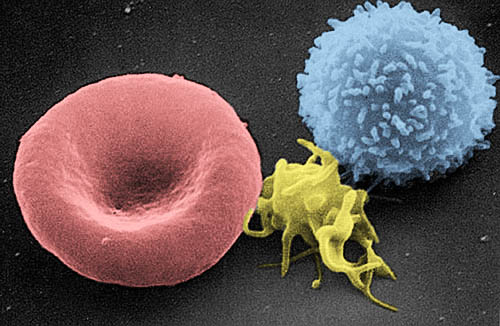
\includegraphics[width=0.4\linewidth]{images/book3/red-cells-nci.jpg}

{\small Sebuah \omterm{def:b1:cell-unit-of-life:cell}{sel} darah merah, sebuah keping darah dan sebuah limfosit
di bawah \omterm{prop:b1:cell-unit-of-life:microscopes}{mikroskop elektron} payar (diberi warna). Bentuk bikonkaf \omterm{def:b1:cell-unit-of-life:cell}{sel}
merahnya ditahan sebuah jala protein di bawah membrannya; ia bertahan
empat bulan diperas menembus kapiler yang lebih sempit daripada dirinya.
Gambar: National Cancer Institute, domain publik.}
\end{omfigure}

\begin{proposition}[Membran adalah dwilapis dan bersifat cair]\label{prop:b1:membranes-transport:evidence}
\omterm{def:b1:membranes-transport:membrane}{Membran plasma} tepat setebal dua molekul lipid, dan komponennya
bergerak di dalam bidangnya.
\end{proposition}
\begin{proof}[Bukti eksperimental]
Gorter dan Grendel (1925) mengekstraksi lipid sejumlah \omterm{def:b1:cell-unit-of-life:cell}{sel} darah merah
yang diketahui dan membentangkannya sebagai selapis tunggal di atas
air: luasnya dua kali total permukaan \omterm{def:b1:cell-unit-of-life:cell}{selnya}, jadi membrannya adalah
sebuah dwilapis. Mikroskopi elektron memperlihatkan tiap membran
sebagai dua garis gelap (kepalanya yang terwarnai) mengapit teras yang
pucat (ekornya), seluruhnya \qty{5}{nm}. Frye dan Edidin (1970)
meleburkan sebuah \omterm{def:b1:cell-unit-of-life:cell}{sel} mencit dengan sebuah \omterm{def:b1:cell-unit-of-life:cell}{sel} manusia yang protein
permukaannya telah ditandai zat warna dua warna: sesudah empat puluh
menit pada \qty{37}{\celsius} kedua warna itu bercampur sempurna pada
\omterm{def:b1:cell-unit-of-life:cell}{sel} hibridnya, dan tidak demikian pada \qty{4}{\celsius}, tempat
lipidnya nyaris padat. Memucatkan setitik \omterm{def:b1:membranes-transport:membrane}{protein membran} yang berpendar
dengan sebuah laser lalu mengamati pendarannya kembali sementara molekul
yang belum pucat berdifusi masuk (FRAP) mengukur difusi menyampingnya:
$\qty{1}{\micro m^2}$ dalam beberapa sekon bagi lipid, lebih lambat bagi
protein, dan nol bagi protein yang tertambat pada \omterm{def:b1:eukaryotic-cell:cytoskeleton}{rangka sel}.
\end{proof}

\begin{definition}[Protein membran]\label{def:b1:membranes-transport:proteins}
\omterm{def:b1:membranes-transport:membrane}{Protein membran} \emph{integral}\index{protein integral} menembus
dwilapis itu dengan satu heliks hidrofob atau lebih dan hanya dapat
diekstraksi dengan deterjen; protein \emph{tepi} terikat pada satu
sisinya. Menurut fungsinya: \emph{pengangkut} (saluran, pembawa,
pompa), \emph{reseptor} yang mengikat sebuah isyarat di luar lalu
bertindak di dalam, \emph{enzim}, \emph{penambat} yang menghubungkan
\omterm{def:b1:eukaryotic-cell:cytoskeleton}{rangka sel} dengan \omterm{def:b1:body-plans-tissues:connective}{matriks ekstrasel}, dan protein \emph{pengenal} yang
membawa gula yang dipakai \omterm{def:b1:cell-unit-of-life:cell}{sel} untuk saling mengenali. Protein adalah
separuh massa sebuah membran yang lazim dan hampir seluruh fungsinya.
\end{definition}

\section{Melintasi membran tanpa bantuan}

\begin{proposition}[Permeabilitas dwilapisnya]\label{prop:b1:membranes-transport:permeability}
\index{permeabilitas}
Sebuah \omterm{def:b1:membranes-transport:membrane}{dwilapis lipid} murni bebas tertembus molekul nonpolar yang kecil
($\mathrm{O_2}$, $\mathrm{CO_2}$, $\mathrm{N_2}$, steroid), cukup
tertembus molekul polar tak bermuatan yang kecil (air, urea, etanol),
buruk tertembus molekul polar yang lebih besar (glukosa, asam amino),
dan praktis tak tertembus ion ($\mathrm{Na^+}$, $\mathrm{K^+}$,
$\mathrm{Cl^-}$, $\mathrm{H^+}$) maupun makromolekul.
Permeabilitasnya membentang dua belas orde besar, dari
$\qty{e-2}{cm/s}$ bagi air sampai $\qty{e-14}{cm/s}$ bagi
$\mathrm{Na^+}$: sebuah teras hidrofob setebal \qty{3}{nm} meloloskan
apa yang larut dalam minyak dan menahan apa yang bermuatan.
\end{proposition}

\begin{theorem}[Hukum difusi Fick]\label{thm:b1:membranes-transport:fick}
\index{hukum Fick}\index{difusi}
Fluks bersih $J$ sebuah zat terlarut melintasi membran seluas $S$ (mol
tiap sekon) sebanding dengan selisih kepekatan di seberangnya:
\[
J = P\,S\,(c_{\text{luar}} - c_{\text{dalam}}),
\]
dengan \emph{koefisien permeabilitas} $P$ (dalam \unit{m/s}) merangkum
koefisien difusi zat terlarut itu di dalam membran, kelarutannya dalam
lipid dan tebal membrannya ($P = DK/\ell$). Difusi tidak memerlukan
energi dan selalu berjalan menuruni gradiennya; ia adalah
\emph{pengangkutan pasif}\index{pengangkutan pasif}.
\end{theorem}
\begin{proof}
Di dalam membran zat terlarut itu berdifusi menuruni profil kepekatan
yang linear dari $Kc_{\text{luar}}$ ke $Kc_{\text{dalam}}$ ($K$ adalah
koefisien partisi antara lipid dan air); hukum pertama Fick dalam
ruahnya, $J/S = -D\,\dd c/\dd x$, memberikan $J/S = DK(c_{\text{luar}} -
c_{\text{dalam}})/\ell$.
\end{proof}

\begin{definition}[Osmosis, potensial air]\label{def:b1:membranes-transport:osmosis}
Yang disebut \emph{osmosis}\index{osmosis} adalah difusi bersih air
melintasi sebuah membran yang meloloskan air tetapi tidak zat
terlarutnya, dari larutan tempat airnya lebih pekat (zat terlarutnya
lebih sedikit) ke larutan tempat airnya kurang pekat. Ia diperikan
\emph{potensial air}\index{potensial air} $\Psi$, yaitu potensial kimia
air yang dinyatakan sebagai sebuah tekanan, bernilai nol bagi air murni
pada tekanan atmosfer:
\[
\Psi = \Psi_s + \Psi_p, \qquad \Psi_s = -RTc_s ,
\]
dengan $\Psi_s$, \emph{potensial zat terlarut}\index{potensial zat terlarut}
, turun bersama kepekatan total zat terlarut $c_s$ (dalam
osmol tiap liter, hukum van 't Hoff) dan $\Psi_p$, \emph{potensial
tekanan}\index{potensial tekanan}, adalah tekanan hidrostatik di atas
tekanan atmosfer. Air berpindah dari $\Psi$ yang lebih tinggi ke yang
lebih rendah. Pada
\qty{25}{\celsius}, $RT = \qty{2.48}{MPa.L/mol}$: a \qty{0.3}{osmol/L}
larutan memiliki $\Psi_s = \qty{-0.74}{MPa}$. Sebuah larutan disebut
\emph{isotonik}\index{isotonik} terhadap sebuah \omterm{def:b1:cell-unit-of-life:cell}{sel} bila tak ada air
yang berpindah bersih, \emph{hipotonik} bila air masuk,
\emph{hipertonik} bila air keluar.
\end{definition}

\begin{omfigure}
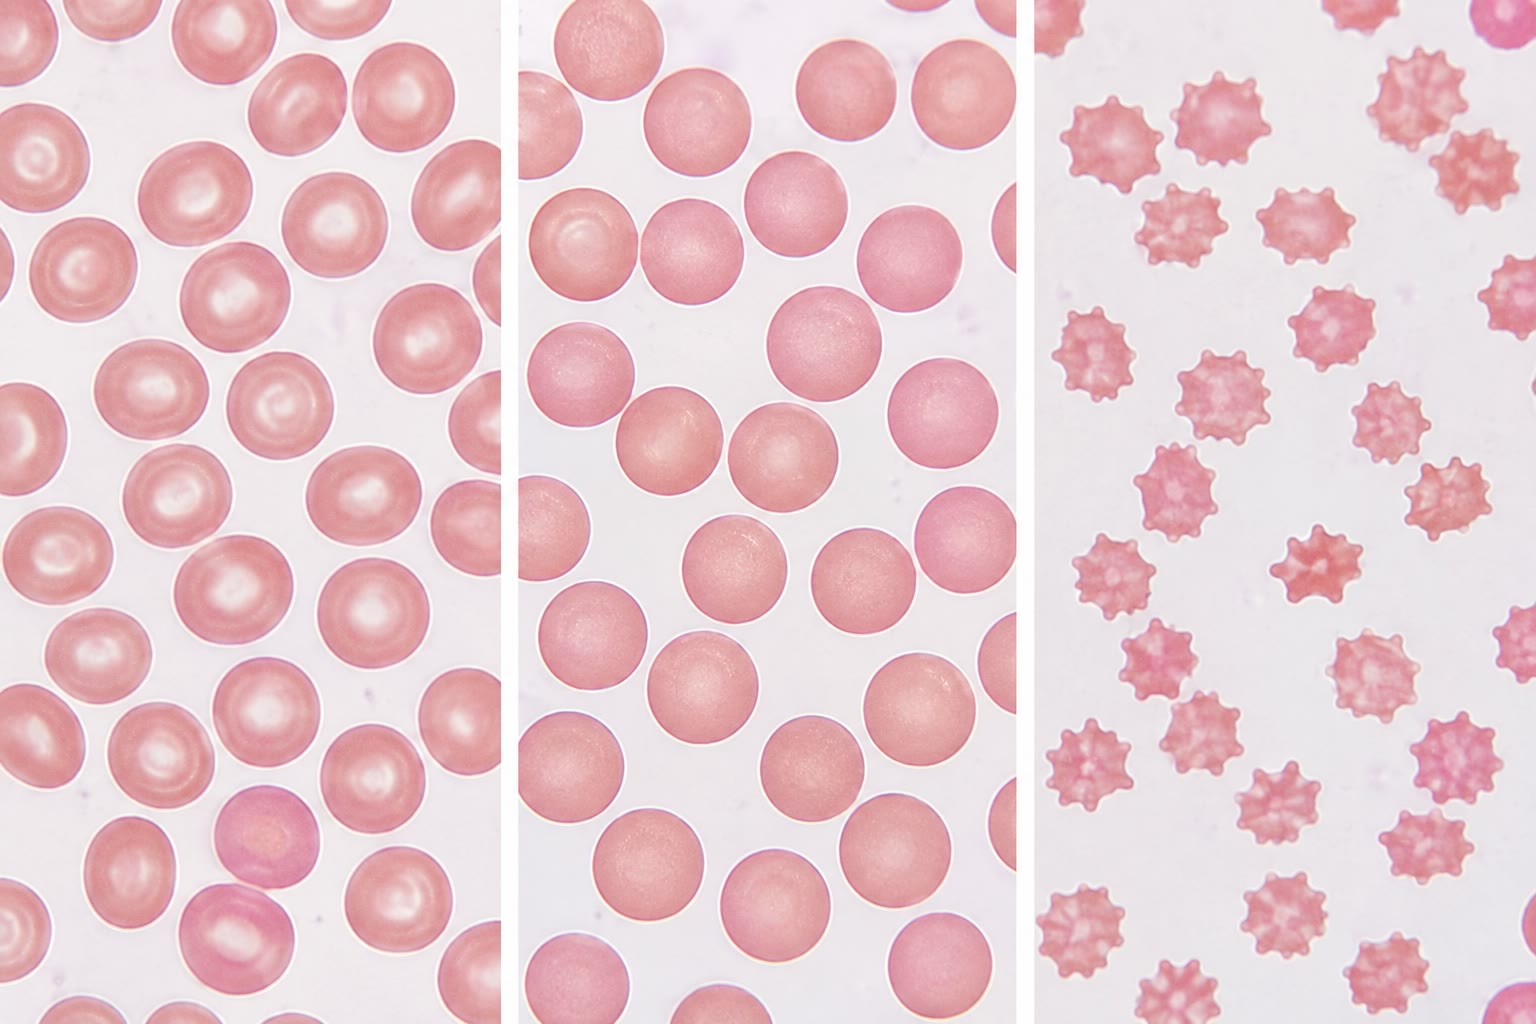
\includegraphics[width=0.78\linewidth]{images/book3/ai/b3-07-red-cells-osmosis.jpg}

{\small \omterm{def:b1:cell-unit-of-life:cell}{Sel} darah merah dalam larutan \omterm{def:b1:membranes-transport:osmosis}{isotonik} (cakram bikonkaf), dalam
larutan hipotonik (membengkak menjadi bola, hampir pecah) dan dalam
larutan hipertonik (mengerut dan berkeriput). Air mengikuti
potensialnya; \omterm{def:b1:cell-unit-of-life:cell}{sel} itu tidak berdinding untuk menahannya.}
\end{omfigure}

\begin{omfigure}
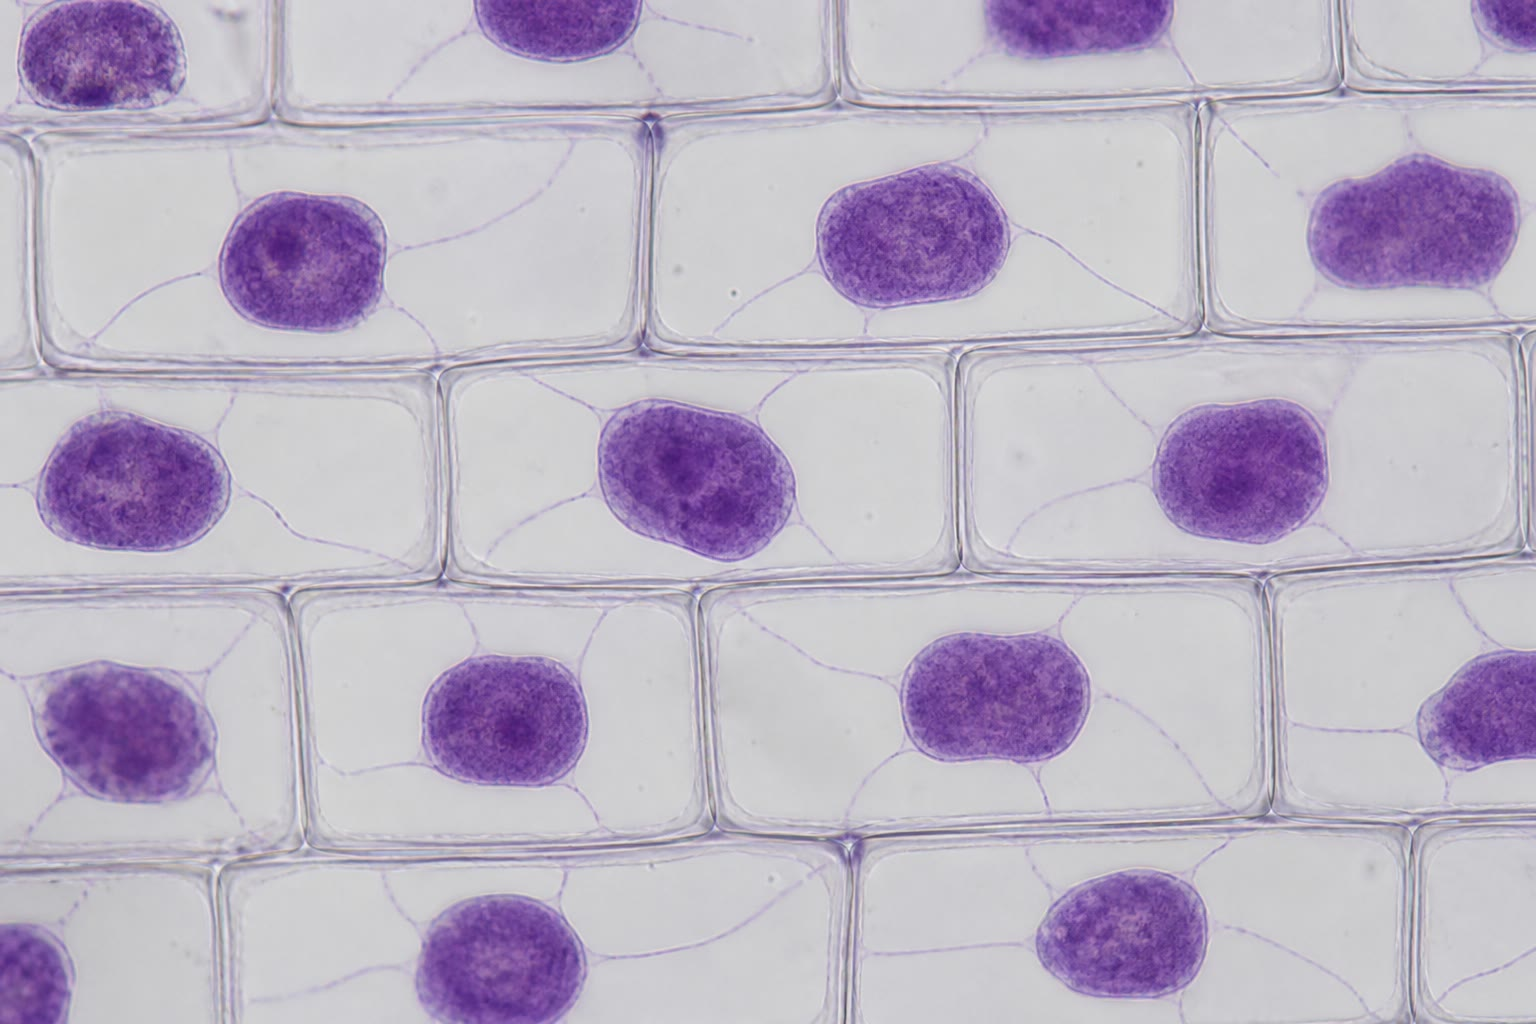
\includegraphics[width=0.6\linewidth]{images/book3/ai/b3-07-plasmolysis.jpg}

{\small Plasmolisis: \omterm{def:b1:flowering-plant-organization:tissues}{epidermis} bawang dalam larutan garam yang pekat.
Protoplas tiap \omterm{def:b1:cell-unit-of-life:cell}{selnya} telah kehilangan air dan menarik diri dari
dindingnya yang kaku, yang tetap berbentuk. Dalam air protoplas itu akan
membengkak kembali menekan dindingnya lalu berhenti, dalam keadaan
menegang.}
\end{omfigure}

\begin{example}[Sebuah sel merah dalam tiga larutan]\label{ex:b1:membranes-transport:redcell}
Plasma adalah \qty{0.3}{osmol/L}: $\Psi_s = \qty{-0.74}{MPa}$ pada kedua
sisinya, tak ada aliran bersih. Dalam air murni ($\Psi = 0$) \omterm{def:b1:cell-unit-of-life:cell}{sel} itu,
yang di dalamnya \qty{-0.74}{MPa}, menyerap air sampai membrannya, yang
hanya sanggup meregang beberapa persen, robek. Dalam garam
\qty{0.6}{osmol/L} ia kehilangan air sampai bagian dalamnya sama
pekatnya, pada separuh volumenya. Sebuah \omterm{def:b1:cell-unit-of-life:cell}{sel} tumbuhan dalam air murni
tidak pecah: seiring masuknya air, dindingnya teregang dan $\Psi_p$ naik
sampai $\Psi_p = -\Psi_s$, \omterm{def:b1:membranes-transport:osmosis}{potensial air} di dalamnya nol, dan alirannya
berhenti dengan \omterm{def:b1:cell-unit-of-life:cell}{sel} itu menegang pada
\qty{0.74}{MPa}.
\end{example}

\begin{method}[Neraca potensial air]\label{met:b1:membranes-transport:psi}
\begin{enumerate}
  \item Ubahlah tiap kepekatan zat terlarut menjadi osmol (sebuah garam
        yang terurai menjadi dua ion dihitung dua kali) lalu hitunglah $\Psi_s =
        -RTc_s$.
  \item Tambahkan suku tekanannya: $\Psi_p = 0$ bagi sebuah larutan
        dalam bejana terbuka atau sebuah \omterm{def:b1:cell-unit-of-life:cell}{sel} hewan, positif bagi \omterm{def:b1:cell-unit-of-life:cell}{sel}
        tumbuhan yang menegang, negatif bagi air yang tertarik di dalam
        sebuah \omterm{def:b1:flowering-plant-organization:tissues}{trakea} \omterm{def:b1:flowering-plant-organization:tissues}{xilem}.
  \item Air mengalir ke arah $\Psi$ yang lebih rendah. Kesetimbangannya
        tercapai ketika kedua $\Psi$ sama: lewat pengenceran isi \omterm{def:b1:cell-unit-of-life:cell}{selnya}
        (\omterm{def:b1:cell-unit-of-life:cell}{sel} hewan), atau lewat naiknya tekanan (\omterm{def:b1:cell-unit-of-life:cell}{sel} tumbuhan).
  \item Bacalah tanda hasilnya sebagai arah alirannya, dan besarnya
        sebagai gaya penggeraknya; laju alirannya juga bergantung pada
        permeabilitas air membrannya, yang dinaikkan seratus kali lipat
        oleh saluran \omterm{def:b1:membranes-transport:transporters}{akuaporin}.
\end{enumerate}
\end{method}

\section{Protein pengangkut}

\begin{definition}[Saluran, pembawa, pompa]\label{def:b1:membranes-transport:transporters}
\emph{Saluran}\index{saluran} adalah \omterm{def:b1:membranes-transport:proteins}{protein integral} dengan sebuah
liang berisi air tempat sebuah ion atau molekul kecil tertentu
berdifusi menuruni gradiennya sampai $10^8$ tiap sekon; banyak di
antaranya \emph{bergerbang}, yang membuka sebagai tanggapan atas sebuah
tegangan, sebuah ligan atau sebuah gaya mekanis.
\emph{Akuaporin}\index{akuaporin} adalah saluran air.
\emph{Pembawa}\index{pembawa} mengikat zat terlarutnya pada satu sisi,
berubah bentuk, lalu melepasnya pada sisi yang lain, paling banyak
seribu kali tiap sekon; pengangkut glukosa \omterm{def:b1:cell-unit-of-life:cell}{sel} darah merah adalah
salah satunya. Saluran dan pembawa yang bekerja menuruni sebuah gradien
menjalankan \emph{difusi terbantu}\index{difusi terbantu}, yang pasif
tetapi memilih dan dapat jenuh. \emph{Pompa}\index{pompa} adalah pembawa
yang menggandengkan pengangkutan sebuah zat terlarut melawan gradiennya
dengan hidrolisis ATP: \emph{pengangkutan aktif
primer}\index{pengangkutan aktif}. \emph{Pompa natrium--kalium}\index{pompa natrium--kalium}
\omterm{def:b1:cell-unit-of-life:cell}{sel} hewan mengekspor tiga $\mathrm{Na^+}$ dan mengimpor
dua $\mathrm{K^+}$ tiap ATP; \emph{pompa proton} pada membran tumbuhan,
jamur dan bakteri mengekspor $\mathrm{H^+}$.
\end{definition}

\begin{omfigure}
\begin{tikzpicture}[font=\footnotesize, >=Stealth, line cap=round]
  % membrane band
  \fill[omDef!15] (0,0) rectangle (13.1,1.2);
  \draw[omDef!60!black] (0,0) -- (13.1,0) (0,1.2) -- (13.1,1.2);
  \node[anchor=east, gray, align=right] at (-0.15,1.5) {sisi luar\\ ($\mathrm{Na^+}$ tinggi,\\ $\mathrm{K^+}$ rendah)};
  \node[anchor=east, gray, align=right] at (-0.15,-0.3) {sitosol\\ ($\mathrm{Na^+}$ rendah,\\ $\mathrm{K^+}$ tinggi)};
  % simple diffusion
  \draw[->, thick, omProp] (1.0,2.0) -- (1.0,-0.8);
  \node[anchor=south, align=center] at (1.0,2.1) {difusi sederhana\\ $\mathrm{O_2}$, $\mathrm{CO_2}$};
  % channel
  \draw[thick, omThm!80!black, fill=omThm!30, rounded corners=2pt] (2.6,-0.2) rectangle (3.0,1.4);
  \draw[thick, omThm!80!black, fill=omThm!30, rounded corners=2pt] (3.3,-0.2) rectangle (3.7,1.4);
  \draw[->, thick, omProp] (3.15,2.0) -- (3.15,-0.8);
  \node[anchor=south, align=center] at (3.15,2.1) {saluran\\ $\mathrm{K^+}$, air};
  % carrier (facilitated)
  \draw[thick, omThm!80!black, fill=omThm!30, rounded corners=5pt] (5.0,-0.3) rectangle (6.0,1.5);
  \draw[->, thick, omProp] (5.5,2.0) -- (5.5,1.55);
  \draw[->, thick, omProp] (5.5,-0.35) -- (5.5,-0.8);
  \node[anchor=south, align=center] at (5.5,2.1) {pembawa\\ glukosa};
  \node[align=center, font=\scriptsize] at (5.5,0.6) {mengikat,\\ membalik};
  % pump
  \draw[thick, omExo!80!black, fill=omExo!30, rounded corners=5pt] (7.5,-0.3) rectangle (8.7,1.5);
  \draw[->, very thick, omExo!80!black] (7.8,-0.8) -- (7.8,2.0);
  \draw[->, very thick, omExo!80!black] (8.4,2.0) -- (8.4,-0.8);
  \node[anchor=south, align=center] at (8.1,2.1) {pompa\\ $3\,\mathrm{Na^+}$ keluar,\\ $2\,\mathrm{K^+}$ masuk};
  \node[anchor=north, align=center, font=\scriptsize] at (8.1,-0.85) {ATP $\to$ ADP};
  % secondary active (symport)
  \draw[thick, omThm!80!black, fill=omThm!30, rounded corners=5pt] (11.0,-0.3) rectangle (12.2,1.5);
  \draw[->, very thick, omProp] (11.3,2.0) -- (11.3,-0.8);
  \draw[->, very thick, omExo!80!black] (11.9,2.0) -- (11.9,-0.8);
  \node[anchor=south, align=center] at (11.6,2.1) {simport\\ $\mathrm{Na^+}$ turun,\\ glukosa naik};
  \node[anchor=north, align=center, font=\scriptsize] at (11.6,-0.85) {aktif sekunder};
  \node[anchor=north west, align=left, gray, font=\scriptsize] at (0,-1.5) {panah jingga: menuruni gradiennya (pasif);\\ hijau: melawannya (aktif)};
\end{tikzpicture}

{\small Lima cara melintas. Difusi sederhana menembus lipidnya; sebuah
saluran dan sebuah pembawa (\omterm{def:b1:membranes-transport:transporters}{difusi terbantu}, menuruni gradiennya);
\omterm{def:b1:membranes-transport:transporters}{pompa natrium--kalium} (\omterm{def:b1:membranes-transport:transporters}{pengangkutan aktif primer}, yang dibayar dengan
ATP); sebuah \omterm{prop:b1:membranes-transport:secondary}{simporter} yang memakai gradien natrium bentukan pompa itu
untuk menyeret glukosa mendaki (\omterm{prop:b1:membranes-transport:secondary}{pengangkutan aktif sekunder}).}
\end{omfigure}

\begin{proposition}[Pengangkutan aktif sekunder]\label{prop:b1:membranes-transport:secondary}
\index{pengangkutan aktif sekunder}
Sebuah gradien yang dibangun sebuah pompa adalah simpanan energi yang
dibelanjakan pembawa lain: sebuah \emph{simporter}\index{simporter}
memindahkan sebuah zat terlarut mendaki dengan menggandengkannya pada
sebuah ion yang menuruni gradiennya searah (pengangkut
natrium--glukosa usus dan ginjal; pengangkut proton--sukrosa floem),
sedangkan sebuah \emph{antiporter}\index{antiporter} menggandengkannya
pada sebuah ion yang bergerak berlawanan arah (penukar
natrium--kalsium). Pada \omterm{def:b1:cell-unit-of-life:cell}{sel} hewan mata uangnya adalah gradien
$\mathrm{Na^+}$; pada tumbuhan, jamur dan bakteri gradien
$\mathrm{H^+}$.
\end{proposition}

\begin{example}[Kinetika menyingkap mekanismenya]\label{ex:b1:membranes-transport:kinetics}
Fluks glukosa ke dalam sebuah \omterm{def:b1:cell-unit-of-life:cell}{sel} merah naik bersama kepekatan di
luarnya, lalu mendatar pada sebuah nilai maksimum, seperti sebuah enzim
(\cref{ch:b1:enzymes}): sebuah pembawa, yang dapat jenuh, dengan $K_m$
sekitar \qty{1.5}{mmol/L}; gula serupa, manosa, bersaing memperebutkannya.
Fluks urea naik sebanding dengan kepekatannya tanpa batas: difusi
sederhana. Fluks glukosa ke dalam \omterm{def:b1:cell-unit-of-life:cell}{sel} usus berhenti ketika natrium
disingkirkan dari lumennya, atau ketika pompanya diracuni ouabain:
\omterm{prop:b1:membranes-transport:secondary}{pengangkutan aktif sekunder}.
\end{example}

\section{Potensial membran}

\begin{definition}[Potensial membran]\label{def:b1:membranes-transport:potential}
Setiap \omterm{def:b1:cell-unit-of-life:cell}{sel} yang hidup memegang sebuah beda potensial listrik di seberang
\omterm{def:b1:membranes-transport:membrane}{membran plasmanya}, yaitu \emph{potensial membran}\index{potensial membran}
$V_m = V_{\text{dalam}} - V_{\text{luar}}$, yang negatif di
dalam: \qty{-70}{mV} pada sebuah \omterm{def:b1:body-plans-tissues:nervous}{neuron}, \qty{-90}{mV} pada sebuah
serabut otot, \qty{-120}{mV} atau lebih pada sebuah \omterm{def:b1:cell-unit-of-life:cell}{sel} tumbuhan. Ia
timbul karena membrannya tertembus secara memilih oleh ion yang
kepekatannya berbeda di seberangnya.
\end{definition}

\begin{theorem}[Persamaan Nernst]\label{thm:b1:membranes-transport:nernst}
\index{persamaan Nernst}\index{potensial kesetimbangan}
Sebuah ion bermuatan $z$ pada kepekatan $c_{\text{luar}}$ dan
$c_{\text{dalam}}$ berada dalam kesetimbangan di seberang membran ---
tanpa fluks bersih, meskipun membrannya tertembus olehnya --- ketika
potensialnya sama dengan \emph{\omterm{thm:b1:membranes-transport:nernst}{potensial kesetimbangannya}}
\[
E_{\text{ion}} = \frac{RT}{zF}\,\ln\frac{c_{\text{luar}}}{c_{\text{dalam}}}
= \frac{\qty{61.5}{mV}}{z}\,\log_{10}\frac{c_{\text{luar}}}{c_{\text{dalam}}}
\quad (\qty{37}{\celsius}).
\]
Bagi $\mathrm{K^+}$ pada \qty{5}{mmol/L} di luar dan \qty{140}{mmol/L}
di dalam, $E_K = 61.5\log(5/140) = \qty{-89}{mV}$; bagi $\mathrm{Na^+}$
pada \qty{145}{} di luar dan \qty{12}{} di dalam, $E_{Na} = \qty{+67}{mV}$.
\end{theorem}
\begin{proof}
Memindahkan satu mol ion itu dari luar ke dalam mengubah energi bebasnya
sebesar jumlah suku kepekatan dan suku listrik:
\[
\Delta G = RT\ln\frac{c_{\text{dalam}}}{c_{\text{luar}}} + zFV_m .
\]
Pada kesetimbangan $\Delta G = 0$, yang memberikan $V_m = (RT/zF)\ln(c_{\text{luar}}/c_{\text{dalam}})$.
Mengubahnya ke logaritma basis sepuluh dan memasukkan $R = \qty{8.314}{J.mol^{-1}.K^{-1}}$,
$T = \qty{310}{K}$, $F = \qty{96485}{C/mol}$ memberikan bentuk numeriknya.
\end{proof}

\begin{proposition}[Asal usul potensial istirahat]\label{prop:b1:membranes-transport:resting}
Membran yang beristirahat jauh lebih tertembus $\mathrm{K^+}$ (lewat
saluran kalium yang terbuka) daripada $\mathrm{Na^+}$; $\mathrm{K^+}$
bocor keluar menuruni gradien kepekatannya, sehingga meninggalkan bagian
dalam yang negatif, sampai tarikan listrik balik hampir mengimbangi
kebocorannya. Karena itu potensial istirahatnya terletak dekat $E_K$,
tertarik sedikit ke arah $E_{Na}$ oleh kebocoran natrium yang kecil
(persamaan Goldman membobot suku Nernst tiap ion dengan
permeabilitasnya). \omterm{def:b1:membranes-transport:transporters}{Pompanya} menopang gradien yang jika tidak akan
dilesapkan kebocoran itu; ia juga menyumbang beberapa milivolt secara
langsung, sebab ia memindahkan tiga muatan keluar bagi dua yang masuk.
\end{proposition}
\begin{proof}[Bukti eksperimental]
Pada sebuah akson cumi-cumi potensial istirahatnya mengikuti $E_K$
ketika kalium di luarnya diragamkan pada rentang yang lebar (sebuah
garis lurus berkemiringan \qty{58}{mV} tiap dekade pada kepekatan
tinggi), dan menyimpang darinya pada kepekatan rendah tepat seperti
yang diramalkan permeabilitas natrium yang kecil. Menghambat pompanya
dengan ouabain hampir tidak mengubah potensialnya selama beberapa
menit, lalu membiarkannya meluruh sepanjang beberapa jam seiring
habisnya gradien itu: potensialnya adalah potensial difusi, sedangkan
pompanya penopang jangka panjangnya.
\end{proof}

\begin{omfigure}
\begin{tikzpicture}
\begin{semilogxaxis}[
  width=0.86\linewidth, height=6.2cm,
  axis x line=bottom, axis y line=left,
  xmin=0.8, xmax=200, ymin=-135, ymax=10,
  xlabel={$\mathrm{K^+}$ luar (\unit{mmol/L})}, ylabel={potensial membran (\unit{mV})},
  xlabel style={font=\small, at={(axis description cs:0.5,-0.12)}, anchor=north},
  ylabel style={font=\small},
  tick label style={font=\small}, xtick={1,10,100}, log ticks with fixed point, ytick={-120,-100,-80,-60,-40,-20,0},
  legend style={font=\small, at={(0.03,0.97)}, anchor=north west, draw=none},
  clip=false,
]
\addplot[thick, dashed, omDef, domain=0.8:200, samples=40] {58*log10(x/140)};
\addlegendentry{Nernst $E_K$ (kemiringan \qty{58}{mV} tiap dekade)}
\addplot[very thick, omThm, domain=0.8:200, samples=60] {58*log10((x+0.01*145)/(140+0.01*12))};
\addlegendentry{terukur: $\mathrm{K^+}$ ditambah kebocoran kecil $\mathrm{Na^+}$}
\draw[dashed, gray] (axis cs:5,-135) -- (axis cs:5,-82);
\node[font=\scriptsize, anchor=west] at (axis cs:5.5,-120) {fisiologis \qty{5}{mmol/L}};
\end{semilogxaxis}
\end{tikzpicture}

{\small Potensial istirahat terhadap kalium luar. Pada kalium yang
tinggi membrannya berlaku sebagai elektrode kalium dan mengikuti garis
Nernst; pada kalium yang rendah kebocoran natrium yang kecil
menariknya di atas
$E_K$.}
\end{omfigure}

\begin{example}[Ke mana energi pompanya pergi]\label{ex:b1:membranes-transport:pumpcost}
Memompa satu $\mathrm{Na^+}$ keluar melawan \qty{12}{} sampai
\qty{145}{mmol/L} dan \qty{-70}{mV} menuntut biaya
$RT\ln(145/12) + F\times 0.070 = 6.4 + 6.8 =
\qty{13.2}{kJ/mol}$; tiga di antaranya, \qty{40}{kJ}, ditambah dua
$\mathrm{K^+}$ masuk pada $RT\ln(140/5) - F\times 0.070 = 8.6 - 6.8 =
\qty{1.8}{kJ/mol}$ masing-masing: \qty{43}{kJ} tiap daur, berhadapan
dengan \qty{50}{kJ} satu ATP pada keadaan seluler. \omterm{def:b1:membranes-transport:transporters}{Pompa} itu bekerja
dekat batas termodinamikanya, dan ia menghabiskan sepertiga ATP seekor
hewan yang berbaring, dua pertiganya di dalam otak.
\end{example}

\section{Pengangkutan ruah}

\begin{proposition}[Pengangkutan vesikel]\label{prop:b1:membranes-transport:vesicles}
Makromolekul dan partikel melintasi \omterm{def:b1:membranes-transport:membrane}{membran plasma} tanpa menembusnya:
lewat \emph{eksositosis}, sebuah vesikel melebur dengan membrannya lalu
mengosongkan diri ke luar; lewat \emph{\omterm{def:b1:eukaryotic-cell:endocytosis}{endositosis}}, membrannya menelan
bahan ke dalam sebuah vesikel (\cref{ch:b1:eukaryotic-cell}). Keduanya
memerlukan ATP, keduanya memindahkan membran maupun isinya, dan keduanya
mempertahankan sisi membrannya. Ketiga rute melintasi sebuah membran ---
menembus lipidnya, menembus sebuah protein, di dalam sebuah vesikel ---
memilih dengan tiga cara: menurut kelarutan, menurut pengenalan molekul,
dan menurut pilihan apa yang ditelan.
\end{proposition}

\begin{example}[Pengantaran kolesterol]\label{ex:b1:membranes-transport:ldl}
Kolesterol mengembara dalam darah di dalam partikel bersalut protein
yang terlalu besar bagi pembawa mana pun. Sebuah \omterm{def:b1:cell-unit-of-life:cell}{sel} yang memerlukan
kolesterol memajang reseptor bagi partikel itu; partikel dan reseptornya
berkumpul dalam sebuah lekuk bersalut, yang lalu menjepit diri, dan
vesikelnya mengantarkan partikel itu ke sebuah \omterm{def:b1:eukaryotic-cell:endomembrane}{lisosom} tempat
kolesterolnya dibebaskan. Seseorang yang reseptornya cacat tidak sanggup
membersihkan partikel itu: kolesterol darahnya berlipat dua dan arterinya
tersumbat pada awal masa dewasa. Satu \omterm{def:b1:membranes-transport:membrane}{protein membran}, satu penyakit.
\end{example}

\section{Latihan}

\begin{exercise}[$\star$]\label{exo:b1:membranes-transport:1}
Perikan \omterm{def:b1:membranes-transport:membrane}{model mosaik cair} dalam empat kalimat: lipidnya, proteinnya,
kecairannya, ketaksetangkupannya.
\end{exercise}

\begin{exercise}[$\star$]\label{exo:b1:membranes-transport:2}
Urutkan $\mathrm{O_2}$, glukosa, $\mathrm{Na^+}$, air dan etanol
menurut permeabilitasnya menembus \omterm{def:b1:membranes-transport:membrane}{dwilapis lipid} murni, dan jelaskan
urutannya.
\end{exercise}

\begin{exercise}[$\star$]\label{exo:b1:membranes-transport:3}
Hitunglah \omterm{def:b1:membranes-transport:osmosis}{potensial zat terlarut} larutan sukrosa \qty{0.1}{mol/L} dan
larutan NaCl \qty{0.1}{mol/L} pada \qty{25}{\celsius}.
\end{exercise}

\begin{exercise}[$\star$]\label{exo:b1:membranes-transport:4}
Hitunglah potensial Nernst $\mathrm{Cl^-}$ pada \qty{120}{mmol/L} di
luar dan \qty{4}{mmol/L} di dalam, pada \qty{37}{\celsius}. Apakah
klorida berada dalam kesetimbangan di dalam \omterm{def:b1:cell-unit-of-life:cell}{sel} pada \qty{-89}{mV}?
\end{exercise}

\begin{exercise}[$\star\star$]\label{exo:b1:membranes-transport:5}
Gorter dan Grendel memakai $\num{4.7e9}$ \omterm{def:b1:cell-unit-of-life:cell}{sel} merah berpermukaan
\qty{100}{\micro m^2} masing-masing dan memperoleh selapis tunggal
lipid seluas \qty{0.92}{m^2}. Hitunglah rasio luas lapisan itu terhadap
permukaan \omterm{def:b1:cell-unit-of-life:cell}{selnya} lalu simpulkan.
\end{exercise}

\begin{exercise}[$\star\star$]\label{exo:b1:membranes-transport:6}
Sebuah \omterm{def:b1:cell-unit-of-life:cell}{sel} tumbuhan memiliki \omterm{def:b1:membranes-transport:osmosis}{potensial zat terlarut} \qty{-0.9}{MPa} dan
\omterm{def:b1:membranes-transport:osmosis}{potensial tekanan} \qty{0.5}{MPa}. \omterm{def:b1:cell-unit-of-life:cell}{Sel} itu ditempatkan dalam sebuah
larutan berpotensial zat terlarut \qty{-0.6}{MPa} di dalam cawan
terbuka. Ke arah mana air berpindah, dan berapa \omterm{def:b1:membranes-transport:osmosis}{potensial tekanan} \omterm{def:b1:cell-unit-of-life:cell}{sel}
itu pada kesetimbangan (anggap \omterm{def:b1:membranes-transport:osmosis}{potensial zat terlarutnya} tidak berubah)?
\end{exercise}

\begin{exercise}[$\star\star$]\label{exo:b1:membranes-transport:7}
Penyerapan glukosa oleh sebuah \omterm{def:b1:cell-unit-of-life:cell}{sel} diukur pada kepekatan luar yang
meningkat: \qtylist{1;2;5;10;20}{mmol/L} memberikan
\qtylist{0.4;0.67;1.0;1.25;1.43}{\micro mol/min}. Tunjukkan bahwa
penyerapannya menjenuh, taksirlah laju maksimumnya dan kepekatan yang
memberikan separuhnya, lalu namailah mekanismenya.
\end{exercise}

\begin{exercise}[$\star\star$]\label{exo:b1:membranes-transport:8}
Jelaskan mengapa potensial istirahat sebuah \omterm{def:b1:cell-unit-of-life:cell}{sel} dekat pada $E_K$ dan
bukan pada $E_{Na}$, dan apa yang akan terjadi padanya bila saluran
natriumnya tiba-tiba terbuka.
\end{exercise}

\begin{exercise}[$\star\star$]\label{exo:b1:membranes-transport:9}
\omterm{prop:b1:membranes-transport:secondary}{Simporter} natrium--glukosa membawa dua $\mathrm{Na^+}$ tiap glukosa.
Dengan $\mathrm{Na^+}$ pada \qty{145}{mmol/L} di luar dan \qty{12}{} di
dalam serta $V_m = \qty{-60}{mV}$, hitunglah energi bebas yang tersedia
dari kedua ion natrium itu dan rasio kepekatan glukosa maksimum
(dalam/luar) yang sanggup dibangun \omterm{prop:b1:membranes-transport:secondary}{simporter} itu pada \qty{37}{\celsius}.
\end{exercise}

\begin{exercise}[$\star\star\star$]\label{exo:b1:membranes-transport:10}
Sebuah \omterm{def:b1:cell-unit-of-life:cell}{sel} didinginkan sampai \qty{4}{\celsius}. Ramalkan, beserta
alasannya, pengaruhnya pada: kecairan membrannya, difusi sederhana
$\mathrm{O_2}$, pompanya, gradien ionnya sepanjang beberapa jam,
\omterm{def:b1:membranes-transport:potential}{potensial membrannya}, dan volume \omterm{def:b1:cell-unit-of-life:cell}{selnya}. (Ingat bahwa protein \omterm{def:b1:cell-unit-of-life:cell}{selnya}
mengerahkan tarikan osmotik yang biasanya diimbangi gradien natriumnya.)
\end{exercise}

\begin{exercise}[$\star\star\star$]\label{exo:b1:membranes-transport:11}
\omterm{def:b1:cell-unit-of-life:cell}{Sel} leburan Frye dan Edidin memperlihatkan pencampuran sempurna protein
permukaannya pada \qty{37}{\celsius} dalam \qty{40}{min}, tidak sama
sekali pada \qty{4}{\celsius}, dan tidak sama sekali pada
\qty{37}{\celsius} ketika sintesis ATP dihambat --- hasil yang terakhir
kemudian terbukti keliru. Sebutkan apa yang disiratkan tiap hasil
tentang mekanisme pencampurannya, dan mengapa versi yang benar
(pencampurannya tidak memerlukan ATP) penting bagi \omterm{def:b1:membranes-transport:membrane}{model mosaik cair}.
\end{exercise}

\begin{exercise}[$\star\star\star$]\label{exo:b1:membranes-transport:12}
``\omterm{def:b1:membranes-transport:potential}{Potensial membran} adalah hasil sampingan gradien ionnya, bukan sesuatu
yang dibangun \omterm{def:b1:cell-unit-of-life:cell}{sel} secara langsung.'' Bahaslah dalam satu paragraf,
dengan \omterm{thm:b1:membranes-transport:nernst}{persamaan Nernst}, pompanya, dan banyaknya ion yang sebenarnya
dibutuhkan untuk memuati membrannya (kapasitansi \qty{1}{\micro F/cm^2}).
\end{exercise}

\section{Soal: Sang Enterosit}

\begin{problem}[{Soal akhir pekan --- sel yang menarik glukosa keluar
dari usus: pompa, simporter, pembawa dan persamaan Nernst, berakhir pada
rasio glukosa tertinggi yang sanggup dibangun sel itu}]
\label{pb:b1:membranes-transport:1}
Sebuah \omterm{def:b1:cell-unit-of-life:cell}{sel} \omterm{def:b1:body-plans-tissues:epithelium}{epitel} usus (enterosit) setinggi \qty{25}{\micro m} dan
selebar \qty{5}{\micro m}; membran apikalnya menghadap lumen, membran
basolateralnya menghadap darah. \omterm{def:b1:eukaryotic-cell:organelle}{Sitosolnya} memegang \qty{12}{mmol/L}
$\mathrm{Na^+}$ dan \qty{140}{mmol/L} $\mathrm{K^+}$; lumen dan darahnya
memegang \qty{145}{mmol/L} $\mathrm{Na^+}$ dan \qty{5}{mmol/L}
$\mathrm{K^+}$. \omterm{def:b1:membranes-transport:potential}{Potensial membrannya} \qty{-60}{mV}. Ambil
$T = \qty{310}{K}$, $R = \qty{8.314}{J.mol^{-1}.K^{-1}}$,
$F = \qty{96500}{C/mol}$, $RT/F = \qty{26.7}{mV}$, dan
$\Delta G_{\text{ATP}} = \qty{-50}{kJ/mol}$ di dalam \omterm{def:b1:cell-unit-of-life:cell}{selnya}.

\medskip
\noindent\textbf{Bagian I --- Gradiennya.}
\begin{enumerate}
  \item Hitunglah potensial Nernst $\mathrm{Na^+}$ dan
        $\mathrm{K^+}$.
  \item Ion mana yang lebih dekat pada kesetimbangan pada
        \qty{-60}{mV}? Apa yang dikatakan hal ini tentang permeabilitas
        istirahatnya?
  \item Hitunglah perubahan energi bebas bagi satu mol $\mathrm{Na^+}$
        yang masuk ke dalam \omterm{def:b1:cell-unit-of-life:cell}{selnya}, dan bagi satu mol $\mathrm{K^+}$
        yang keluar.
  \item Hitunglah biaya energi bebas satu daur pompa ($3\,\mathrm{Na^+}$
        keluar, $2\,\mathrm{K^+}$ masuk) lalu bandingkan dengan energi
        satu ATP. Berapa efisiensinya?
  \item \omterm{def:b1:membranes-transport:transporters}{Pompanya} hanya terdapat pada membran basolateralnya. Jelaskan
        mengapa penempatan ini diperlukan agar \omterm{def:b1:cell-unit-of-life:cell}{selnya} sanggup
        memindahkan glukosa dari lumen ke darah.
\end{enumerate}

\medskip
\noindent\textbf{Bagian II --- Glukosa mendaki.}
Membran apikalnya membawa sebuah \omterm{prop:b1:membranes-transport:secondary}{simporter} yang memasukkan satu glukosa
bersama dua $\mathrm{Na^+}$; membran basolateralnya membawa sebuah
pembawa glukosa (\omterm{def:b1:membranes-transport:transporters}{difusi terbantu}).
\begin{enumerate}[resume]
  \item Hitunglah energi bebas yang dilepaskan dua $\mathrm{Na^+}$ yang
        masuk ke dalam \omterm{def:b1:cell-unit-of-life:cell}{selnya}.
  \item Tuliskan energi bebas yang dibutuhkan untuk memindahkan satu
        glukosa dari lumen (kepekatan $c_L$) ke \omterm{def:b1:eukaryotic-cell:organelle}{sitosol} ($c_C$).
  \item Pada batas \omterm{prop:b1:membranes-transport:secondary}{simporternya} keduanya sama. Hitunglah rasio maksimum
        $c_C/c_L$.
  \item Bila lumennya turun ke \qty{0.1}{mmol/L} glukosa pada akhir
        penyerapannya, kepekatan \omterm{def:b1:eukaryotic-cell:organelle}{sitosol} berapa yang masih sanggup
        dipertahankan \omterm{prop:b1:membranes-transport:secondary}{simporter} itu?
  \item Glukosa darah adalah \qty{5}{mmol/L}. Jelaskan bagaimana
        glukosa meninggalkan \omterm{def:b1:cell-unit-of-life:cell}{selnya} ke dalam darah tanpa energi
        tambahan apa pun.
  \item Mengapa \omterm{prop:b1:membranes-transport:secondary}{simporternya} ditempatkan pada membran apikal dan
        pembawanya pada membran basolateral, dan bukan sebaliknya?
  \item Larutan rehidrasi oral bagi kolera memuat glukosa dan garam.
        Jelaskan, dari \omterm{prop:b1:membranes-transport:secondary}{simporternya}, mengapa glukosa itu membuat garamnya
        --- dan airnya --- terserap.
\end{enumerate}

\medskip
\noindent\textbf{Bagian III --- Menghitung lalu lintasnya.}
\omterm{def:b1:cell-unit-of-life:cell}{Sel} itu menyerap \qty{2e-15}{mol} glukosa tiap sekon.
\begin{enumerate}[resume]
  \item Hitunglah $\mathrm{Na^+}$ yang masuk tiap sekon lewat
        \omterm{prop:b1:membranes-transport:secondary}{simporternya}, dan banyaknya daur pompa tiap sekon yang
        dibutuhkan untuk mengeksporinya.
  \item Hitunglah ATP yang dibelanjakan tiap sekon bagi ekspor itu, dan
        fraksi glukosa terserap yang harus direspirasi untuk
        membayarnya (sekitar 30 ATP tiap glukosa).
  \item Tiap \omterm{prop:b1:membranes-transport:secondary}{simporter} berdaur \qty{50}{} kali tiap sekon. Berapa
        banyak \omterm{prop:b1:membranes-transport:secondary}{simporter} yang dibutuhkan membran apikalnya? Membran
        apikalnya seluas \qty{25}{\micro m^2} dengan mikrovili yang
        melipatgandakannya \qty{20}{} kali: hitunglah kerapatan
        \omterm{prop:b1:membranes-transport:secondary}{simporternya} tiap mikrometer persegi.
  \item $\mathrm{Na^+}$ yang masuk membawa air secara \omterm{def:b1:membranes-transport:osmosis}{osmosis}. Dua
        $\mathrm{Na^+}$ dan satu glukosa, beserta $\mathrm{Cl^-}$ yang
        menyertainya, adalah empat osmol; \omterm{def:b1:cell-unit-of-life:cell}{sel} itu menjaga
        osmolaritasnya pada \qty{0.3}{osmol/L}. Hitunglah volume air
        yang harus mengikuti zat terlarutnya tiap sekon, dan waktu yang
        dibutuhkannya untuk melipatduakan volume \omterm{def:b1:cell-unit-of-life:cell}{sel} itu seandainya
        airnya tidak keluar lewat membran basolateralnya.
  \item Hitunglah banyaknya molekul air yang diserap tiap molekul
        glukosa (\qty{18}{g/mol}, massa jenis \qty{1}{g/mL}).
\end{enumerate}

\medskip
\noindent\textbf{Bagian IV --- Memuati membrannya.}
Membrannya adalah sebuah kapasitor \qty{1}{\micro F/cm^2}.
\begin{enumerate}[resume]
  \item Hitunglah luas membran \omterm{def:b1:cell-unit-of-life:cell}{sel} itu (ambil sebuah kotak
        \qty{25}{\micro m} kali \qty{5}{\micro m} kali
        \qty{5}{\micro m} tanpa mikrovili) dan kapasitansinya.
  \item Hitunglah muatan yang dibutuhkan untuk menahan \qty{-60}{mV}
        dan banyaknya ion bervalensi satu yang diwakilinya.
  \item Hitunglah banyaknya kelebihan ion tiap mikrometer persegi
        membran yang diwakili hal ini.
  \item Hitunglah banyaknya ion $\mathrm{K^+}$ di dalam \omterm{def:b1:cell-unit-of-life:cell}{selnya}, dan
        fraksi yang harus keluar untuk memuati membrannya. Beri
        tanggapan.
  \item \omterm{def:b1:membranes-transport:transporters}{Pompanya} memindahkan muatan bersih ke luar pada tiap daurnya.
        Dengan memakai pertanyaan 13, hitunglah arus yang dibawanya dan
        perubahan potensial yang akan dihasilkannya dalam satu sekon
        seandainya tak ada yang lain bergerak. Mengapa potensialnya
        sesungguhnya tidak melonjak liar?
  \item Sebuah obat menghambat pompanya. Ramalkan, berurutan, perubahan
        gradien natriumnya, penyerapan glukosanya, \omterm{def:b1:membranes-transport:potential}{potensial membrannya}
        dan volume \omterm{def:b1:cell-unit-of-life:cell}{selnya}.
  \item Sebuah obat menghambat saluran kaliumnya sebagai gantinya.
        Ramalkan perubahan potensial istirahatnya.
  \item Nyatakan hasilnya: rasio kepekatan glukosa maksimum yang
        sanggup dibangun enterosit itu, dan kedua \omterm{def:b1:membranes-transport:membrane}{protein membran} yang
        memungkinkannya.
\end{enumerate}
\end{problem}
